\section{Metadata Analysis - Topical Prevalence and Content}
\label{Metadata Analysis - Topical Prevalence and Content}

\subsection{Topical Prevalence: Method of Composition and Direct Assessment}
\label{Covariate-level Topic Analysis}

We now proceed to analyze the relationship between metadata information (i.e., document-level covariates) and topic proportions. We specify topical prevalence as 
\begin{align}
\mu_{d,k} = \boldsymbol{x_d}^T \boldsymbol{\gamma}_k= \gamma_{k,\text{party}_d} + \gamma_{k,\text{state}_d} + f_k(\text{t}_d) + g_k(\text{struct}_d), \label{prevalence}
\end{align} 
for all documents $d = 1,\dots,D$, and for all topics $k = 1,\dots,K$, where 
\begin{align*}
g_k(\text{struct}_d) = g_{k}^{(1)}(\text{GDP}_d)+g_{k}^{(2)}(\text{unemployment}_d)+g_{k}^{(3)}(\text{immigrants}_d)+g_{k}^{(4)}(\text{votes}_d). 
\end{align*} 
That is, the political party and federal state of the respective parliamentarian associated with a document are specified as simple categorical dummy effects, while date and electoral-district structural covariates (GDP per capita, unemployment rate, percentage of immigrants, and the 2017 vote share) are modeled as additive smooth functions.

Note that approximate inference implies replacing $\mu_{d,k}$ with $\lambda_{d,k}$, i.e., with the mean of the approximate Gaussian posterior $q(\eta_{d,k})$. The estimates of $\boldsymbol{\Gamma} = [\boldsymbol{\gamma}_1 | \dots | \boldsymbol{\gamma}_K]$ are updated in a Bayesian linear regression during each iteration of the EM algorithm in the M-step; for details see \cite{roberts2013structural}, p.\ 993.

While topical prevalence does has an effect on the estimated topic proportions, the exact specification of topical prevalence does not. Both estimated topic proportions and heldout likelihood are in general only marginally affected by the specific choice of the functional form. However, completely removing topical prevalence, in which case the model reduces to a CTM, does result in different topic proportions, as we show in section \ref{Two-step Approach: CTM}. Since evaluation metrics such as held-out likelihood are mostly unaffected by the exact choice of topical prevalence and because the computational cost of fitting an STM is rather high, automatic model selection methods with respect to topical prevalence are not available. A reasonable specification of topical prevalence therefore relies on the domain knowledge of the researcher.

There exist different approaches to study the relationship between topic proportions and prevalence covariates. One possibility is to directly assess the estimates $\hat{\boldsymbol{\Gamma}}$ and $\hat{\boldsymbol{\Sigma}}$ generated by the STM. Since the document-level topic proportions $\boldsymbol{\theta}_d$ follow a logistic normal distribution (with median $\boldsymbol{\mu}_d$ and covariance parameters $\boldsymbol{\Sigma}$), interpretation of the results can be difficult, since the logistic normal distribution is not easily accessible. Nonetheless, we can still visualize the relationship between a topic and a prevalence covariate, fixing other covariates at their median (for categorical variables the majority vote is used).

Alternatively, the estimated topic proportions can be used as dependent variable of a new regression on prevalence covariates. However, in contrast to a standard regression setting, in this case the dependent variable has been estimated itself before the regression is performed. Instead of simply using the maximum-a-posteriori (MAP) estimates of $\boldsymbol{\theta}_d$ as the dependent variable, having access to the posterior distribution of the topic proportions, we can account for the uncertainty of the dependent variable. This can be achieved by employing a sampling procedure known as the method of composition in the social sciences  (\citealp{tanner2012tools}, p.\ 52). This procedure is implemented in the \textit{stm} package through its function \textit{estimateEffect}.

In the following, we first introduce the method of composition. We discuss its implementation in the \textit{stm} package and provide alternative regression approaches based on the method of composition. Subsequently, we evaluate the relationship between prevalence covariates and topic proportions by directly assessing the estimates $\hat{\boldsymbol{\Gamma}}$ and $\hat{\boldsymbol{\Sigma}}$, as outlined above, and compare the results of the two approaches.\\
\\
\noindent \textbf{Method of Composition} \vspace{10px}

Let $\boldsymbol{\theta}_{(k)}:=(\theta_{1,k}, \dots, \theta_{D,k})^T \in [0,1]^{D}$ denote the proportions of the $k$-th topic for all $D$ documents. As stated, we want to perform a regression of these topic proportions $\boldsymbol{\theta}_{(k)}$ on prevalence covariates $\boldsymbol{X} \in \mathbb{R}^{D \times P}$. The true topic proportions are unknown, but the STM produces an estimate of the approximate (variational) posterior of $\boldsymbol{\theta}_{(k)}$. A "na{\"\i}ve" approach would be to regress the estimated mode of the approximate posterior distribution on $\boldsymbol{X}$. However, this approach neglects much of the information contained in the posterior distribution. 

Instead, \cite{roberts2016model} employ a Monte Carlo sampling technique established by \cite{treier2008democracy}, which is known as the "method of composition" (\citealp{tanner2012tools}, p.\ 52) in the social sciences. This method is implemented in the R package \textit{stm} via the function \textit{estimateEffect}. The idea is to repeatedly sample $\boldsymbol{\theta}_{(k)}^*$ from their approximate posterior distribution and subsequently perform a regression for each sampled $\boldsymbol{\theta}_{(k)}^*$ on $\boldsymbol{X}$ in order to take into account the uncertainty in $\boldsymbol{\theta}_{(k)}^*$.

Before we describe this method, we want to demonstrate how sampling $\boldsymbol{\theta}_{(k)}^*$ can be achieved. First, for all documents we sample the unnormalized topic proportions $\boldsymbol{\eta}^* := [\boldsymbol{\eta}^*_1 | \dots | \boldsymbol{\eta}_D^*]$ from the approximate posterior $q(\boldsymbol{\eta}) = \prod_d q(\boldsymbol{\eta}_d)$, to subsequently apply the softmax $\boldsymbol{\theta}^* := [\boldsymbol{\theta}^*_1 | \dots | \boldsymbol{\theta}^*_D] = \text{softmax}(\boldsymbol{\eta}^*)$ (element-wise, i.e., for each of the K-dimensional columns of topic proportions) and select the $k$-th column of $\boldsymbol{\theta}^*$ (which we denote as $\boldsymbol{\theta}_{(k)}^*$). To be precise, for all $d \in {1, \dots, D}$, $q(\boldsymbol{\eta}_d)$ is a normal distribution, which emerges from the Laplace approximation within variational inference; for details see \cite{roberts2016model}, pp.\ 992-993. We denote the approximate posterior of topic proportions as $q(\boldsymbol{\theta}_{(k)} | \boldsymbol{X}, \boldsymbol{W})$, in order to emphasize that the parameters of the posterior distribution are learned from the observed data, i.e.\ prevalence covariates $\boldsymbol{X}$ and words $\boldsymbol{W}$ (note that we have not included any content variables $\boldsymbol{Y}$).

The method of composition applied in the STM, inspired by \cite{treier2008democracy}, can now be described by the following iteration, which is repeated $m$ times:
\begin{enumerate}
\item Sample $\boldsymbol{\theta}^*_{(k)}$ from the variational posterior $q(\boldsymbol{\theta}_{(k)} | \boldsymbol{X}, \boldsymbol{W})$.
\item Run a regression model with response $\boldsymbol{\theta}^*_{(k)}$ and covariates $\boldsymbol{X}$ to obtain an estimate $\hat{\boldsymbol{\xi}}^*$ of regression coefficients $\boldsymbol{\xi}^*$ and covariance matrix of $\hat{\boldsymbol{\xi}}^*$, $\hat{\boldsymbol{V}}^*_{\xi}$.
\item Sample $\tilde{\boldsymbol{\xi}}^*$ from $F(\hat{\boldsymbol{\xi}}^*, \hat{\boldsymbol{V}}^*_{\xi})$, where $F$ denotes the (asymptotic) distribution of $\hat{\boldsymbol{\xi}}^*$.
\end{enumerate}

In the case of \cite{treier2008democracy}, the regression model employed is a Cox regression, where estimators for the regression coefficients are asymptotically normally distributed (i.e., $F$ is a multivariate normal distribution).

The idea of the method of composition is that the samples $\tilde{\boldsymbol{\xi}}^*$ take into account the uncertainty in $\boldsymbol{\theta}_{(k)}$. Additionally, the third step is performed in order to take into account the uncertainty regarding the regression estimation. Visualization of topic-metadata relationship then occurs as follows: For a (new) observation $\boldsymbol{x}_{\text{pred}}$, one can plot $\boldsymbol{x}_{\text{pred}}$ vs. the sampled predicted responses with $\boldsymbol{x}_{\text{pred}}^T \tilde{\boldsymbol{\xi}}_i^*$ as linear predictor, for all $i \in \{1,\dots,m\}$. The empirical mean and other quantities of interest, such as credible intervals, are then calculated using the $m$ sampled response values.

While we agree with the approach of performing Monte Carlo sampling of topic proportions in order to integrate over these latent variables, we have several concerns, especially regarding the specific application of the method of composition in the STM (and the accompanying R package).
\begin{enumerate}
\item \textbf{Problem 1}: In the R package \textit{stm}, the regression model employed in step 2 is an ordinary least squares (OLS) regression; however OLS is not appropriate to model (sampled) proportions, which are constrained to the interval (0,1).
\item \textbf{Problem 2}: A general problem with the method of composition is the mixing of Bayesian and frequentist methods. For instance, \cite{treier2008democracy} state that the sampled regression coefficients can be considered a sample from the posterior of regression coefficients. However, the way the method of composition is presented, we do \textit{not} perform a Bayesian regression and thus regression coefficients do not follow any distribution (only the \textit{estimators} of regression coefficients do); instead, regression coefficients are assumed to be fixed (unknown) parameters from a frequentist perspective. From a Bayesian perspective, the sampled $\tilde{\boldsymbol{\xi}}^*$ can only be considered a sample from the posterior of $\boldsymbol{\xi}$ in some regression models, however, with very questionable (uniform) prior assumptions. After having obtained the samples $\tilde{\boldsymbol{\xi}}^*$, inference of parameters is conducted in a classical Bayesian manner, e.g., calculating the empirical mean via averaging.
\item \textbf{Problem 3}: Separate modeling of topic proportions neglects topic interdependence caused by the (multivariate) logistic normal distribution assumed within the generative process of the STM.
\end{enumerate}
In the following we further discuss these problems and propose alternative approaches.

\subsubsection{Problem 1: Implementation via OLS in the \textit{stm} package}

\noindent As stated, the R package \textit{stm} implements an OLS regression through its \textit{estimateEffect} function. This approach ignores that the sampled topic proportions are restricted to $(0,1)$. As expected, using this framework we frequently observe predicted proportions outside of $(0,1)$:\\

\begin{figure}[h!]
  \centering
  \captionsetup{justification=centering,margin=2cm}
  \begin{subfigure}[b]{0.4\linewidth}
    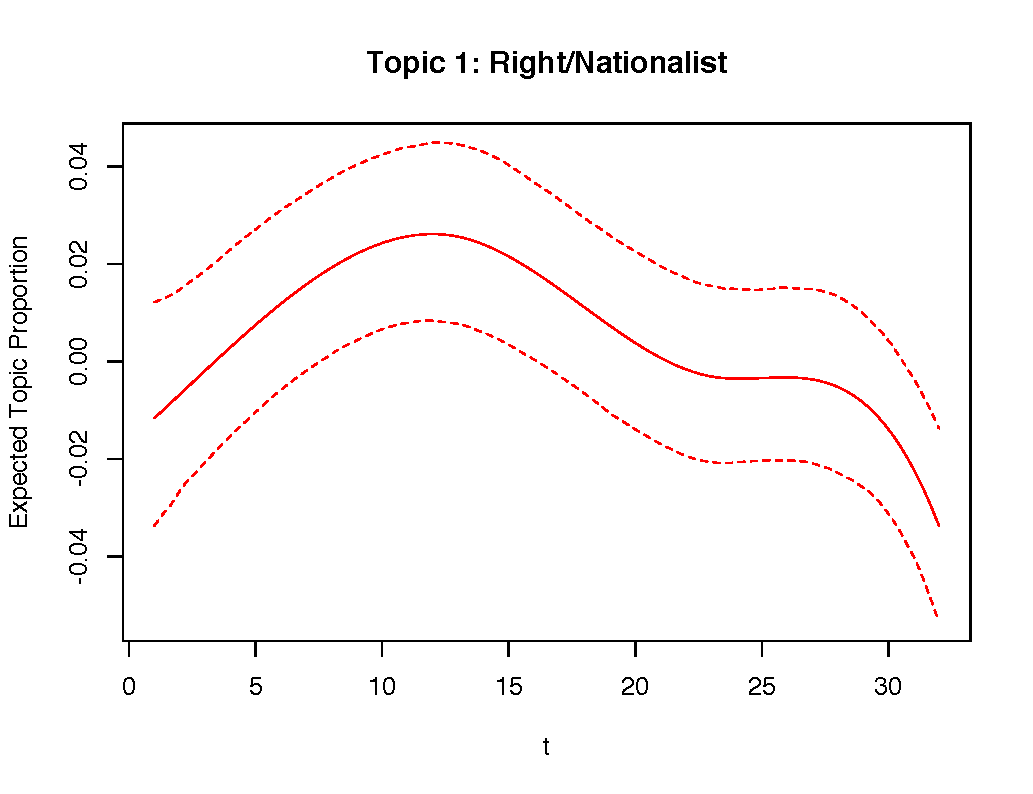
\includegraphics[width=\linewidth]{../plots/5_1/estEffect_topic1.pdf}
  \end{subfigure}
  \begin{subfigure}[b]{0.4\linewidth}
    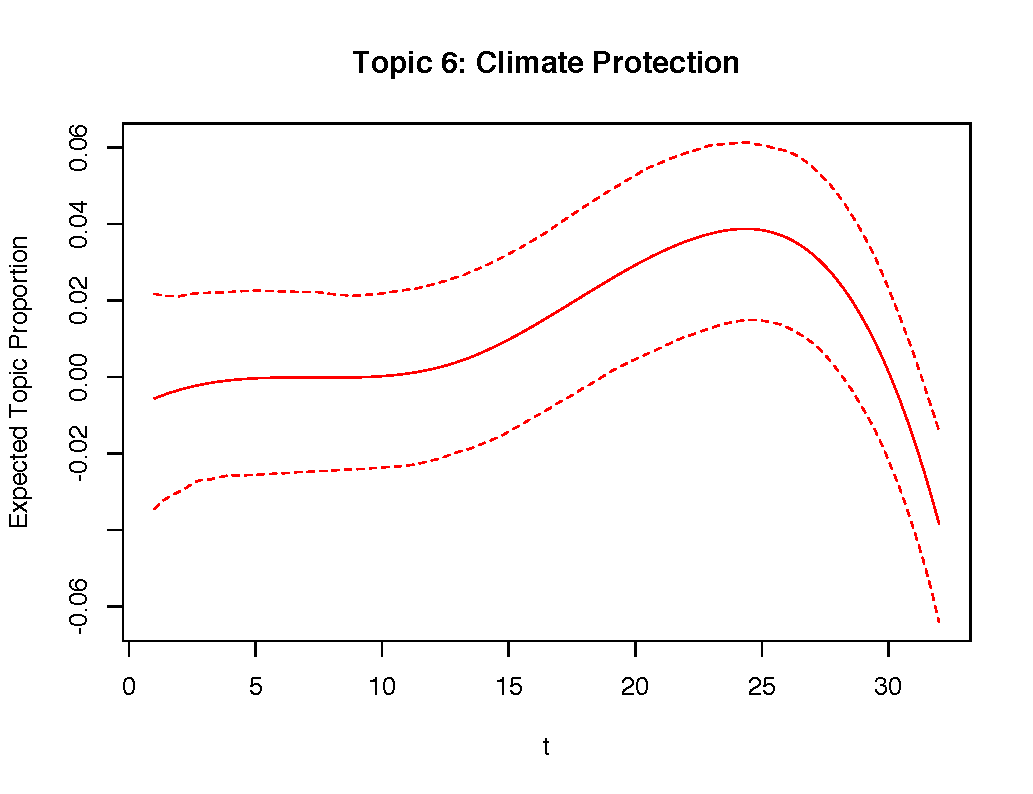
\includegraphics[width=\linewidth]{../plots/5_1/estEffect_topic6.pdf}
  \end{subfigure}\\
  \caption{Estimated prevalence of topics 1 and 6 over time, generated using \textit{estimateEffect} from the \textit{stm} package}
  \label{fig:estEffect_topic16}
\end{figure}
\noindent \textbf{Alternative implementation} \vspace{10px}

\noindent We can attempt to improve the approach employed within the \textit{stm} package by replacing the OLS regression with a regression model that assumes a dependent variable in the interval $(0,1)$. As shown by \cite{atchison1980logistic}, a distribution that can be used to approximate a logistic normal distribution is the Dirichlet distribution. However, note that the Dirichlet distribution assumes less interdependence among components than implied by the logistic normal distribution, as discussed in section \ref{Theoretical Framework}. In case of the Dirichlet distribution the univariate marginal distributions are beta distributions. One possibility is thus to perform a separate beta regression for each topic proportion on $\boldsymbol{X}$. 

As an alternative approximation we can employ a quasibinomial generalized linear model (GLM). The $k$-th topic can be understood as one of two classes, with the remaining topics forming the alternative class. To match the underlying logistic normal distribution more closely, the quasi-likelihood furthermore allows for a flexible variance specification. 

Note that the distribution of regression coefficient estimators is asymptotically normal for both the beta regression (\citealp{ferrari2004beta}, p.\ 17) and the quasibinomial GLM (\citealp{fahrmeir2007regression}, p. 285). In both cases, we use a logit-link. \\
\\
\noindent \textbf{Visualization} \vspace{10px}

\noindent We now apply the method of composition, based on either a beta regression or a quasibinomial GLM, in order to visualize covariate effects. Here we only visualize the results obtained by the quasibinomial GLM; the results of the beta regression, which show similar trends, are found in the appendix. Setting the number of simulations to 100, we sample regression coefficients $\tilde{\boldsymbol{\xi}}^*_1, \dots, \tilde{\boldsymbol{\xi}}^*_{100}$. When visualizing the impact of a particular covariate, all other covariates are held at their median (or majority vote, if categorical), in line with the methodology employed in the \textit{stm} package.

We exemplarily illustrate the relationship between covariates and topic proportions for topic 4 ("Social/Housing") and topic 6 ("Climate Protection"). For smooth effects, it is important to recall that their borders are inherently unstable, which is why one should refrain from (over-)interpreting them. For both continuous and categorical variables, black lines indicate the mean and the shaded area represents 95\% credible intervals.

\begin{figure}[h!]
  \centering
  \captionsetup{justification=centering,margin=2cm}
  \begin{subfigure}[b]{0.49\linewidth}
    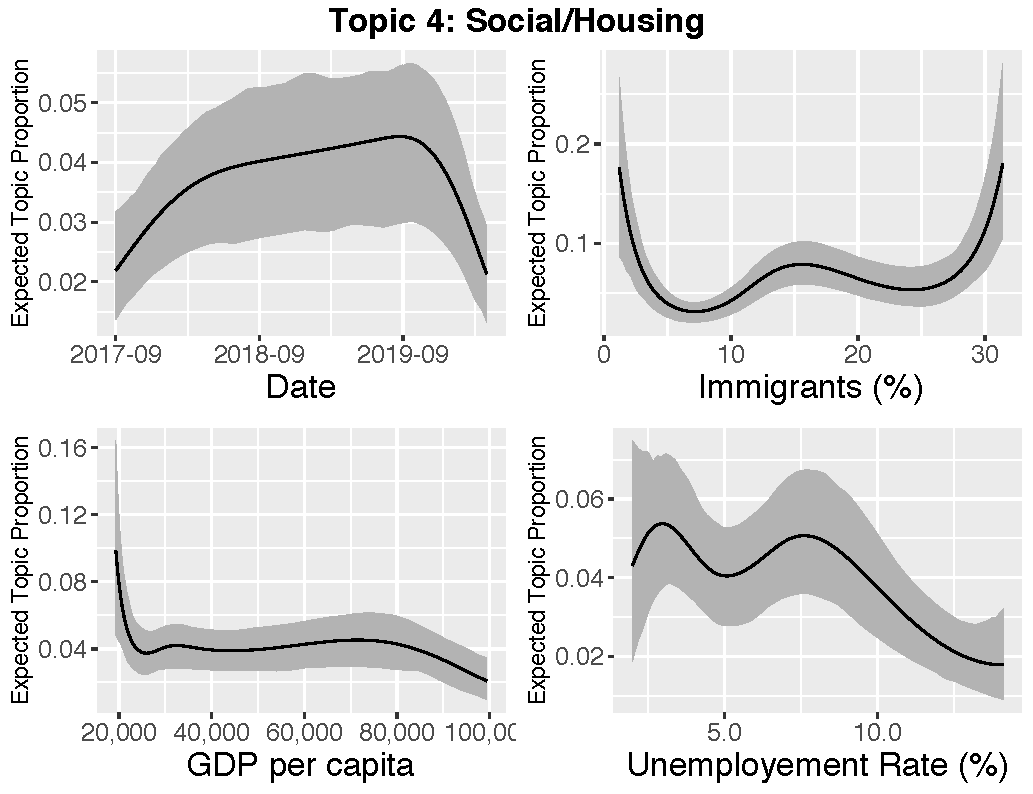
\includegraphics[width=\linewidth]{../plots/5_1/quasi_t4_cont.pdf}
  \end{subfigure}
  \begin{subfigure}[b]{0.49\linewidth}
    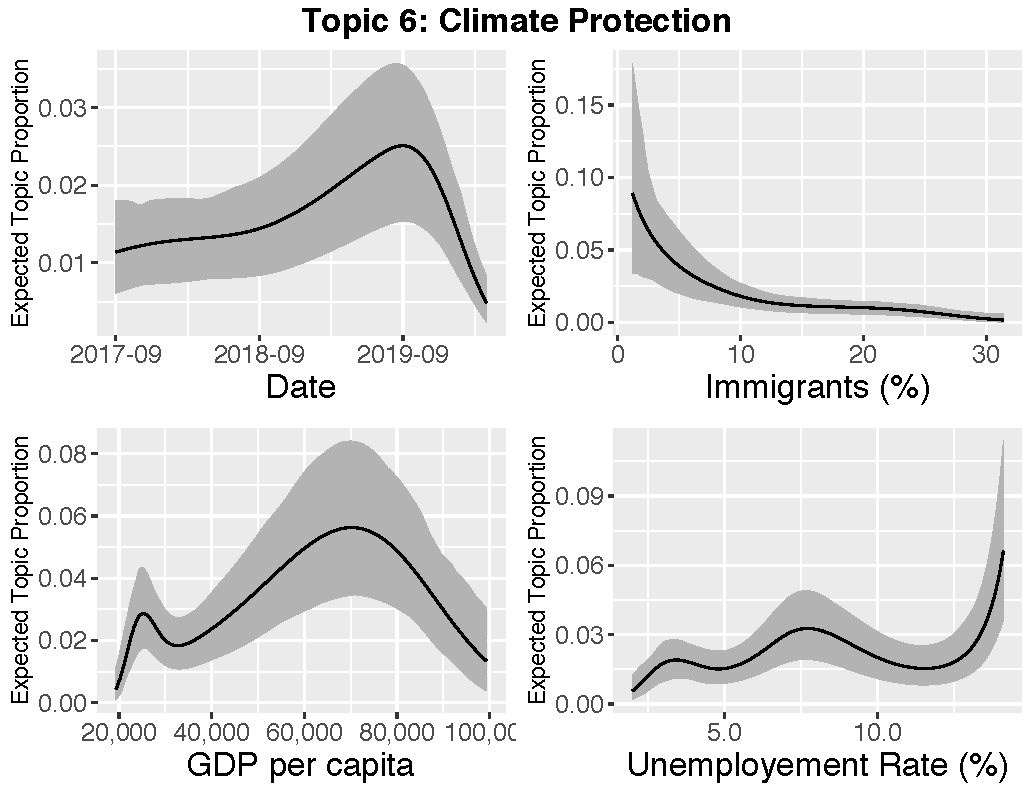
\includegraphics[width=\linewidth]{../plots/5_1/quasi_t6_cont.pdf}
  \end{subfigure}
  \caption{Mean and 95\% credible intervals for smooth effects, obtained using a quasibinomial GLM.}
  \label{fig:quasi_t46_cont}
\end{figure}

\begin{figure}[h!]
  \centering
  \captionsetup{justification=centering,margin=2cm}
  \begin{subfigure}[b]{0.49\linewidth}
    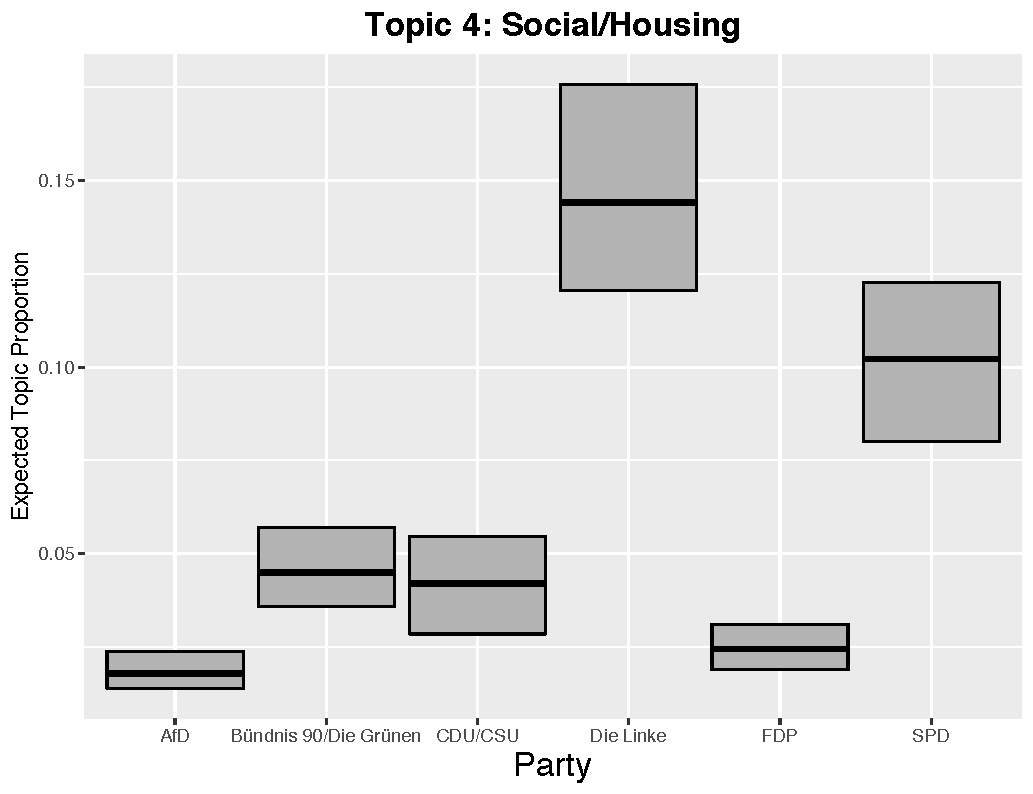
\includegraphics[width=\linewidth]{../plots/5_1/quasi_t4_cat.pdf}
  \end{subfigure}
  \begin{subfigure}[b]{0.49\linewidth}
    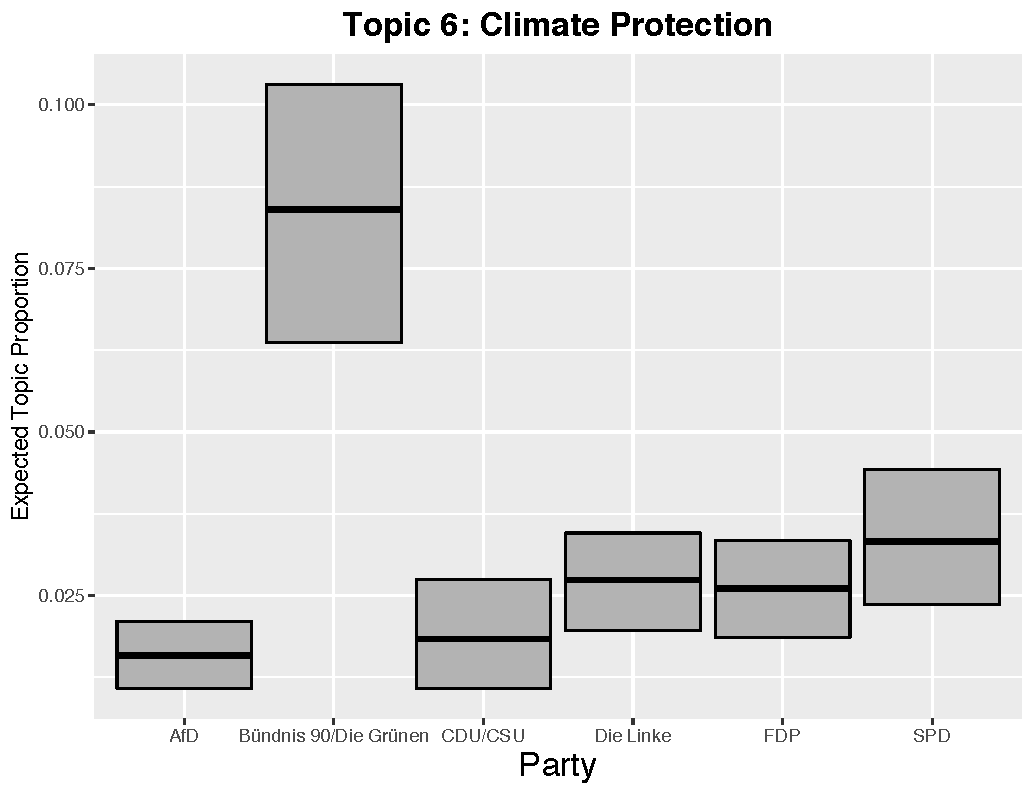
\includegraphics[width=\linewidth]{../plots/5_1/quasi_t6_cat.pdf}
  \end{subfigure}
  \caption{Mean and 95\% credible intervals for different political parties, obtained using a quasibinomial GLM.}
  \label{fig:quasi_t46_cat}
\end{figure}

For topic 4, "Social/Housing", we observe that most continuous variables have a small effect in absolute terms: the absolute variation in topic proportion across the covariate domains merely amounts to 4\%, compared to 8\% for topic 6. For most covariates the trend is rather ambiguous. Somewhat surprisingly, a very high unemployment rate is negatively linked to topic 4.

The effect of the political party on the relevance assigned to the topic "Social/Housing" is very much in line with a priori expectations: the left party and social democrats have the highest topical prevalence (15\% and 10\%, respectively), and the nationalist party the lowest (2\%).

For the smooth effects of topic 6, we observe its prevalence peaks in September 2019, corresponding to month $t=25$, decreasing afterwards. The absolute changes in topic proportions over time are rather small (around 3\%). The percentage of immigrants within an electoral district shows a negative relation with topic 6. Furthermore, topic 6 tends to be discussed more frequently in mid-income electoral districts than in high- or low-income districts. Finally, the link to the unemployment rate is somewhat ambiguous, although generally positive.

Regarding the relationship between the political party and the prevalence of topic "Climate Protection", we find high topical prevalence for the green party, as expected. Similar to the smooth effects, total variation in topic proportions across parties amounts to approximately 8\%.

Finally, the graph below shows a summary comparison of topical prevalence across all parties, for topics "Right/Nationalist", "Climate Protection" and "Social/Housing". The results are generally consistent with expectations. The proportions of topics "Climate Protection" and "Social/Housing" vary between 2\% and 9\% and between 2\% and 15\%, respectively. For topic 1, "Right/Nationalist", note how topical prevalence for the AfD party amounts to more than 40\%, implying that more than 40\% of the total content tweeted by AfD party members is about right-wing/nationalist issues, particularly immigration; for all other parties, topic 1 is rather marginal below 3\%.

\begin{figure}[h!]
  \centering
  \captionsetup{justification=centering,margin=2cm}
  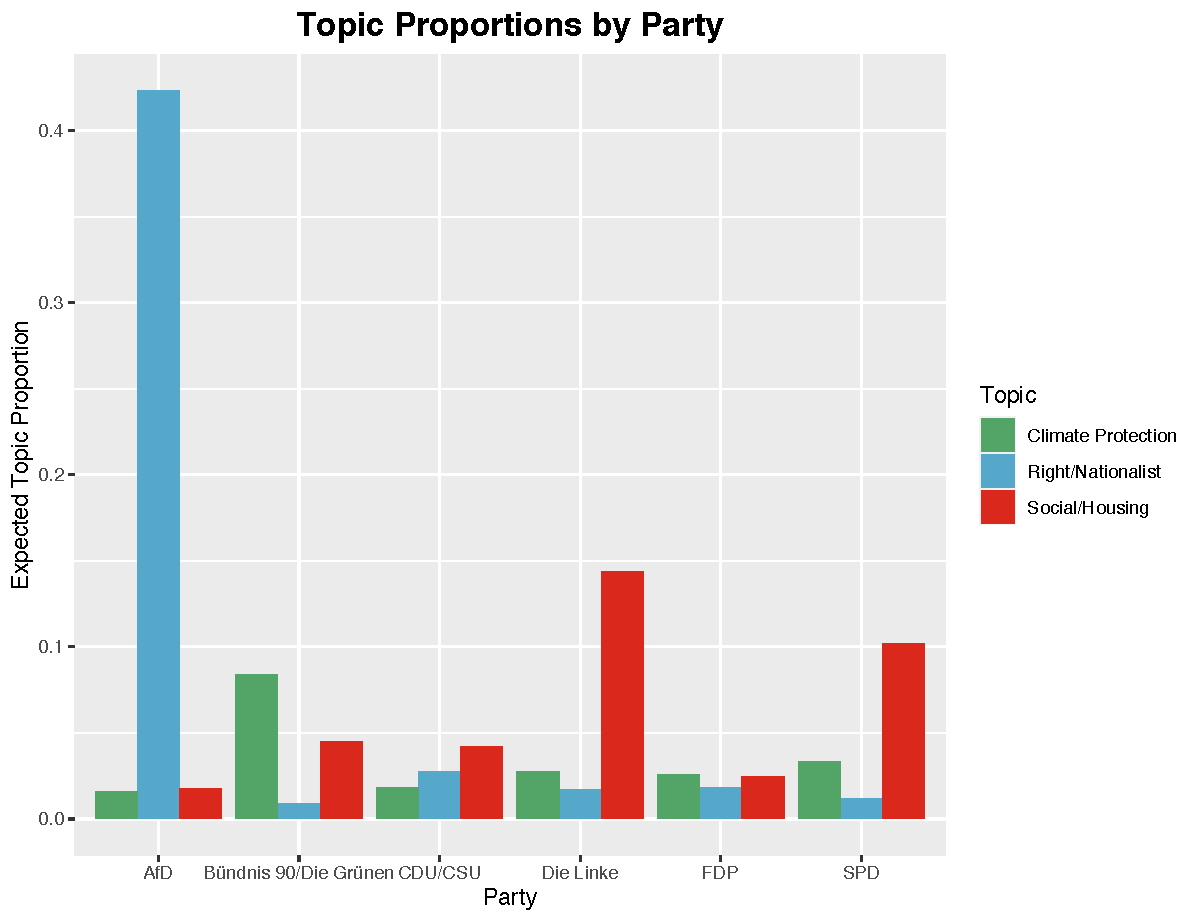
\includegraphics[scale = 0.5]{../plots/5_1/quasi_t146_cat.pdf} \\
  \caption{Topical prevalence by political party for topics 1, 4, and 6.}
  \label{fig:quasi_t146_cat}
\end{figure}

\subsubsection{Problem 2: Mixing of Bayesian and Frequentist Approach}

The regression employed within the method of composition is framed as a \textit{frequentist} regression. However, \cite{treier2008democracy} and the authors of the STM consider $\tilde{\boldsymbol{\xi}}^*$ as samples from the (marginal, i.e., integrated over latent topic proportions) posterior of regression coefficients. In case of an ordinary linear regression this is, however, only true by assuming uniform priors for $\boldsymbol{\xi}$. In general, the mixing of the Bayesian and the frequentist framework within the method of composition is not well-founded theoretically. This is especially the case when employing an \textit{asymptotic} distribution of regression coefficient estimators from the frequentist regression framework, as is the case for the model considered by \cite{treier2008democracy}, the GLM and the beta regression.

Furthermore, note that uncertainty from previous plots is with respect to the prediction of the mean of topic proportions. However, it is not obvious why this is preferable when the objective is to \textit{explore} the topical structure. In particular, the uncertainty with respect to the predicted mean does \textit{not} reflect variation of topic proportions in the data. When exploring the topic-metadata relationship, it might in fact be more instructive to examine the (predicted) variation of topic proportions among individuals at different covariate values.\\
\\
\noindent \textbf{Alternative implementation} \vspace{10px}

Due to these concerns, we propose to replace the (frequentist) regression in the second step of each iteration of the method of composition with an explicit Bayesian regression. In particular, in case of a Bayesian regression we can sample proportions from the respective posterior predictive distribution at the end of each step of the method of composition (i.e., conditioning on previously sampled $\boldsymbol{\theta}_{(k)}^*$) at different covariate values $\boldsymbol{x}_{\text{pred}}$. This allows us to display the (predicted) variation of topic proportions at different covariate levels. Furthermore, the calculation of empirical quantities of interest, such as the mean, now occurs within a fully Bayesian framework, allowing for sound interpretations.

Specifically, in order to adequately model topic proportions we employ a Bayesian beta regression with normal priors centered around zero. Depicting the results from the described procedure (that is, sampling from the posterior predictive distribution at the end of each iteration of the method of composition) in Figure \ref{fig:stanbeta}, we find that the empirical mean is mostly in line with results from our previous analyses. However, since "uncertainty" is now with respect to the variation of (predicted) topic proportions in the data - and not with respect to the prediction of their mean - 95\% credible intervals differ starkly compared to the previous section. In general, we observe that in all cases there seem to be some individuals with rather extreme topic proportions. This corresponds well to what we observe when directly examining the estimated topical structure of the STM in a descriptive manner. For instance, in section \ref{Hyperparameter Search and Model Fitting} we saw that the estimated proportion of topic 1 for MP Martin Hess amounted to 98.86\% in June 2018. We observe such high variation likewise for other topics and covariate values. The fully Bayesian approach allows for a precise exploration of the distribution of topic proportions at different covariate values. The mid panel of Figure \ref{fig:stanbeta} tells us - for instance - that, based on the discovered topical structure, we can expect a lower variation of proportions among parliamentarians for topic 6 in districts with a large share of immigrants. If desired, we could also predict other quantiles of interest. In our view, this approach allows for a much more intuitive exploration of the latent space of topic proportions with respect to different metadata dimensions. 

\begin{figure}[h!]
    \centering
     \captionsetup{justification=centering,margin=2cm}
  \begin{subfigure}[b]{0.3\linewidth}
    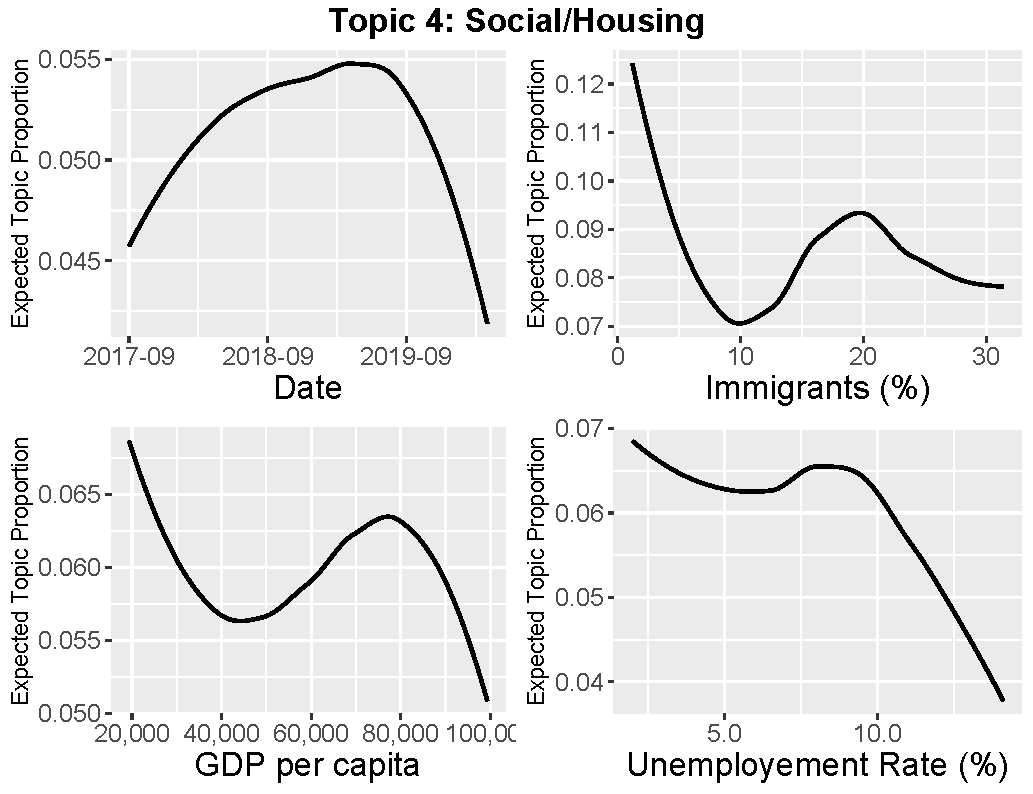
\includegraphics[width=\linewidth]{../plots/5_1/stanbeta_t4_without_credible.pdf}
  \end{subfigure}
  \begin{subfigure}[b]{0.3\linewidth}
    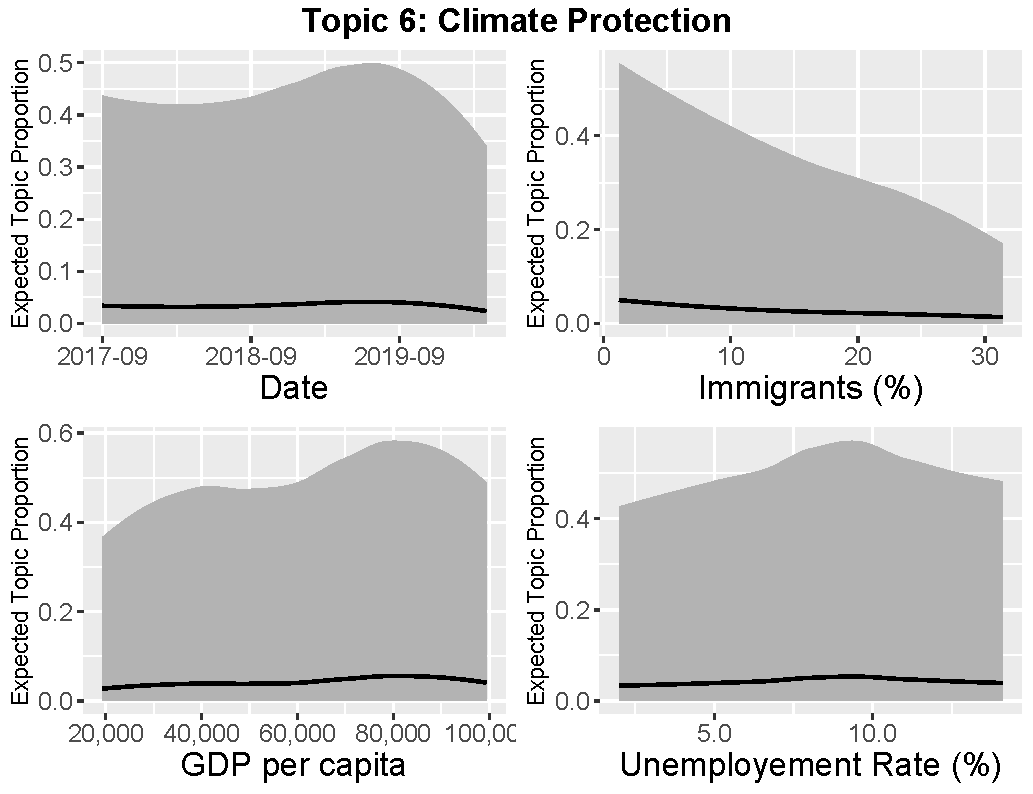
\includegraphics[width=\linewidth]{../plots/5_1/stanbeta_t6_with_credible.pdf}
  \end{subfigure}
  \begin{subfigure}[b]{0.3\linewidth}
    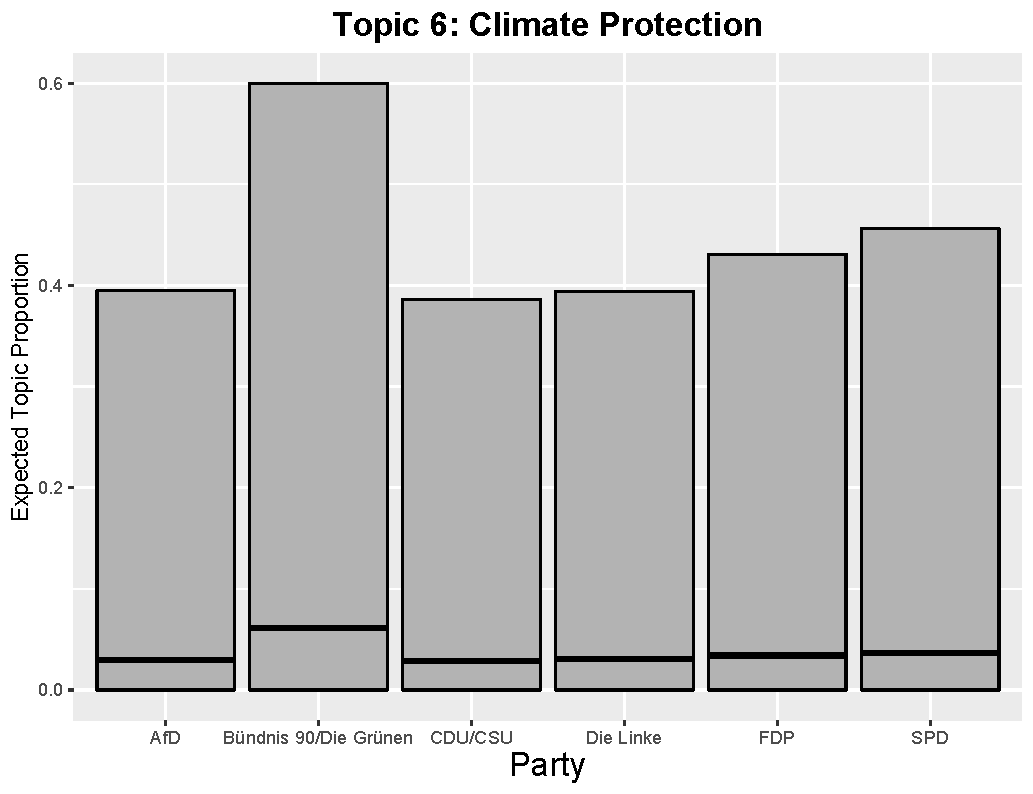
\includegraphics[width=\linewidth]{../plots/5_1/stanbeta_t6_cat.pdf}
  \end{subfigure}
  \caption{Smooth effects without credible intervals (left), smooth effects with credible intervals (center), and effect of the political party (right). Samples from the posterior predictive distribution of topic proportions within the method of composition.}
  \label{fig:stanbeta}
\end{figure}

\subsubsection{Problem 3: Univariate Modeling of Topic Proportions}
\label{Direct assessment}

The STM being an extension of the correlated topic model (CTM), it is assumed that the topic proportions follow a logistic normal distribution, such that $\boldsymbol{\theta}_d \sim \text{LogisticNormal}_{K-1}(\boldsymbol{\Gamma}^T\boldsymbol{x}_d^T, \boldsymbol{\Sigma})$. Within the CTM, the Dirichlet distribution of the LDA has been replaced with a logistic normal distribution, in order to allow for a joint dependence among topics. Therefore, as mentioned above, separately modeling topic proportions is a simplification. 

In order to examine the relation of prevalence covariates and topic proportions considering the joint dependence among latter ones, we can attempt to directly use the output produced by the STM: inference within the STM involves finding the maximum-a-posteriori (MAP) estimate $\hat{\boldsymbol{\Gamma}}$ and the maximum likelihood estimate $\hat{\boldsymbol{\Sigma}}$. 

In order to get an impression of how the assumed generative process of topic proportions in the STM behaves, we can plug the estimates $\hat{\boldsymbol{\Gamma}}$ and $\hat{\boldsymbol{\Sigma}}$ into the logistic normal distribution and visualize sampled values from this distribution. Given a new observation $\boldsymbol{x}_{\text{pred}}$, we can sample $\boldsymbol{\theta}_d^*$ from $\text{LogisticNormal}_{K-1}(\hat{\boldsymbol{\Gamma}}^T\boldsymbol{x}_{\text{pred}}^T, \hat{\boldsymbol{\Sigma}})$ by:

\begin{enumerate}
\item Drawing $\boldsymbol{\eta}_d^* \sim \mathcal{N}_{K-1}(\hat{\boldsymbol{\Gamma}}^T\boldsymbol{x}_{\text{pred}}^T, \hat{\boldsymbol{\Sigma}})$ and setting $\boldsymbol{\eta}^*_{d,K} = 0$.
\item Mapping to the simplex, i.e., for all $k = 1,\dots,K$: $\theta_{d,k}^* = \frac{\exp(\eta^*_{d,k})}{\exp(\sum_{i=1}^{K} \eta^*_{d,i})}$.
\item Setting $\boldsymbol{\theta}_d^* := (\theta_{d,1}^*, \dots \theta_{d,K}^*)^T$.
\end{enumerate}

We repeated the above steps 1000 times for each input value of a selected variable, while fixing other variables at their median, and obtained the empirical mean as well as 95\% credible intervals. Plotting the results, we observe that the mean shows a similar trend to our previous analyses. 
\begin{figure}[h!]
    \centering
     \captionsetup{justification=centering,margin=2cm}
  \begin{subfigure}[b]{0.3\linewidth}
    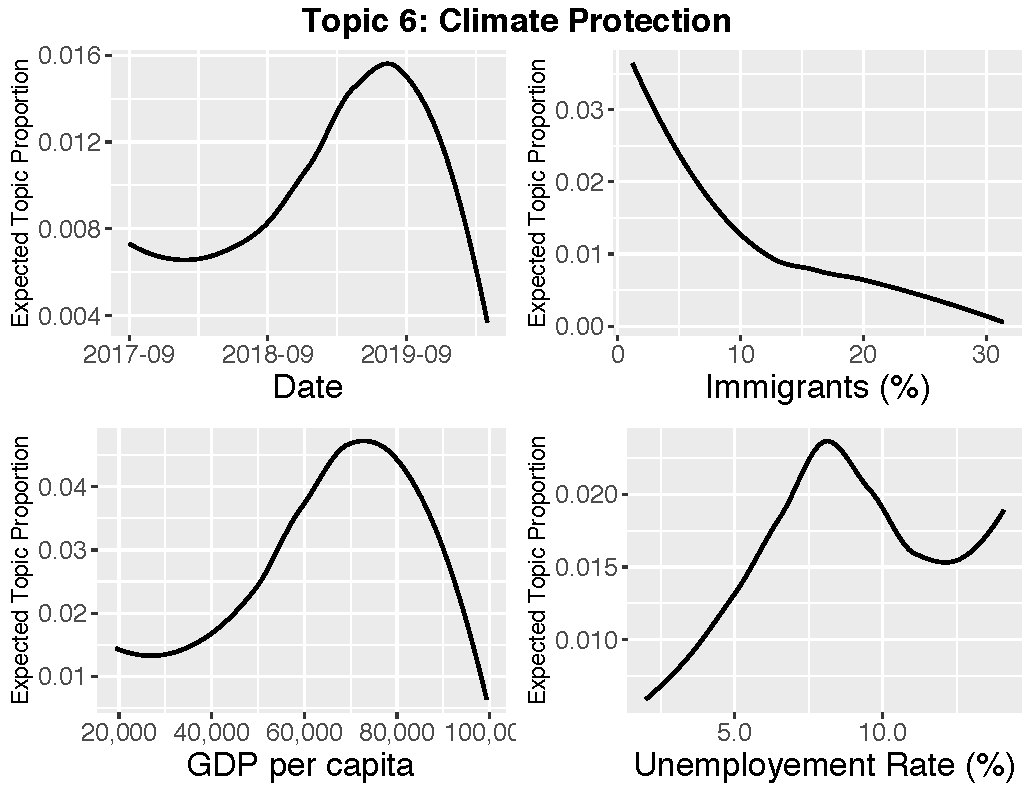
\includegraphics[width=\linewidth]{../plots/5_1/direct_t6_without_credible.pdf}
  \end{subfigure}
  \begin{subfigure}[b]{0.3\linewidth}
    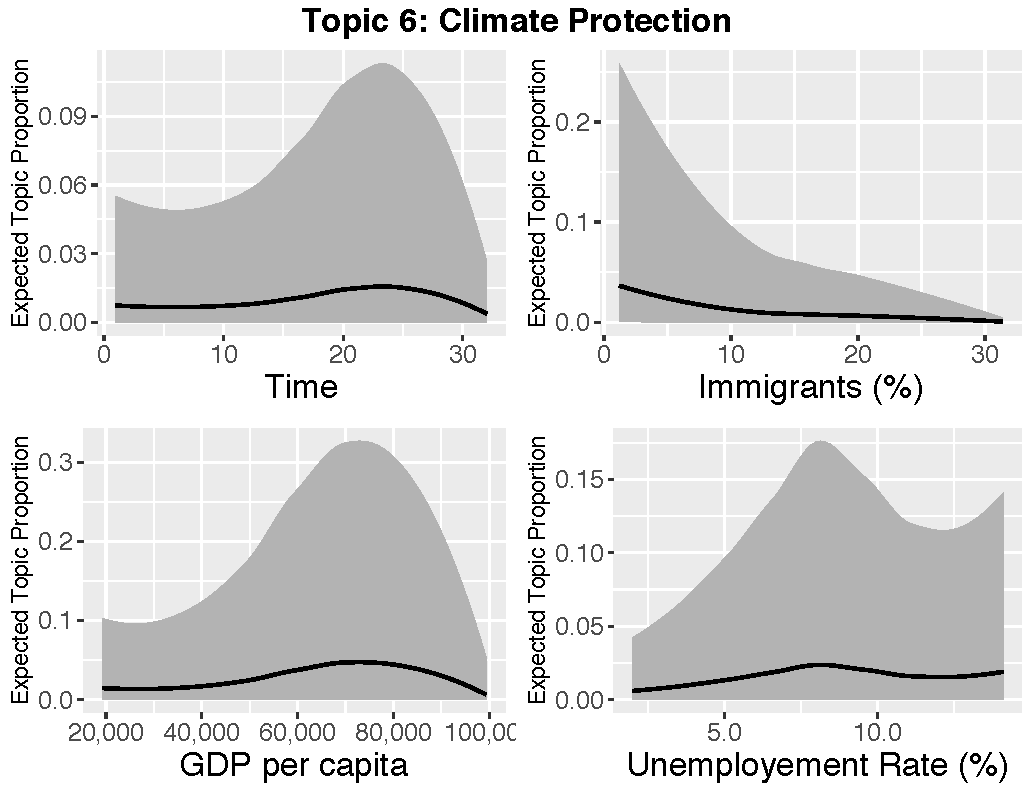
\includegraphics[width=\linewidth]{../plots/5_1/direct_t6_with_credible.pdf}
  \end{subfigure}
  \begin{subfigure}[b]{0.3\linewidth}
    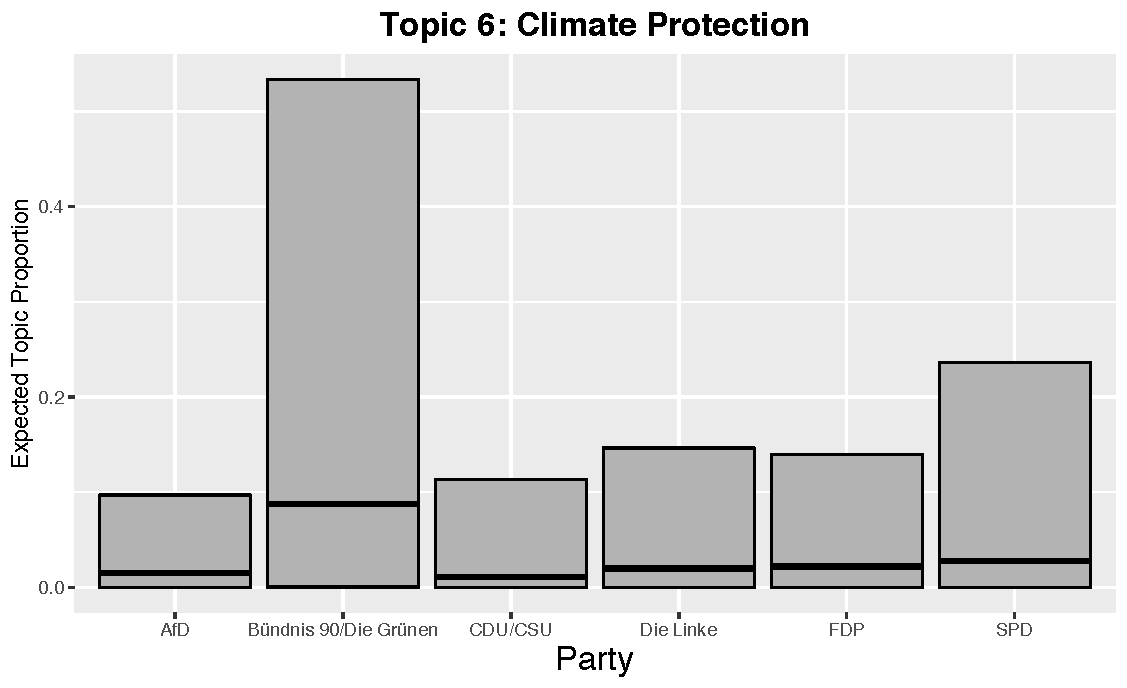
\includegraphics[width=\linewidth]{../plots/5_1/direct_t6_cat.pdf}
  \end{subfigure}
  \caption{Smooth effects without credible intervals (left), smooth effects with credible intervals (center), and effect of the political party (right).}
  \label{fig:directassessment}
\end{figure}

As in the fully Bayesian regression approach, the variation is again with respect to the topic proportions in the data (i.e., not with respect to the predicted mean). Compared to the fully Bayesian approach from the previous section, the variation we observe is much lower. This is due to the fact that plugging in $\hat{\boldsymbol{\Gamma}}$ and $\hat{\boldsymbol{\Sigma}}$ is a "na{\"i}ve" approach. In order to get a more realistic picture, we would have to first sample prevalence parameters from their posterior, and subsequently plug these samples into the logistic normal distribution, yielding samples from the posterior predictive distribution of topic proportions. This would likely result in a variation on the scale of the results obtained using the fully Bayesian regression approach. Unfortunately, sampling of prevalence parameters is not possible using the R package \textit{stm}. 

